% ================================================================
%  CHAPTER 2 - REQUIREMENTS SPECIFICATIONS
% ================================================================
\chapter{Requirements Specifications}

\section*{Introduction}
\addcontentsline{toc}{section}{Introduction}

This chapter formalizes the requirements analysis of the Deterministic Enterprise AI Orchestration Platform. It identifies the system actors, catalogues functional and non-functional requirements, and models interactions through UML use case diagrams. The requirements defined here directly inform the microservices decomposition and Kubernetes deployment strategy detailed in Chapter~3.


% ──────────────────────────────────────────────────────────────────
\section{Identification of Actors}
% ──────────────────────────────────────────────────────────────────

Three actors interact with the platform, each operating at a different architectural layer:

\begin{itemize}
    \item \textbf{End User} - An authenticated enterprise user who submits AI requests through the chat interface. They select intents, choose sensitivity levels, and receive real-time streamed responses. They have no access to administrative functions.

    \item \textbf{Administrator} - A privileged user responsible for configuring the orchestration layer. They manage intent-to-service mappings, define governance policies, set token quotas, deploy edge security plugins, and monitor platform health through a dedicated admin portal.

    \item \textbf{Kong Gateway} - A secondary, non-human actor. The API gateway automatically mediates all inbound traffic by enforcing rate limiting, IP restriction, CORS policies, and JWT validation before forwarding requests to the FastAPI backend.
\end{itemize}


% ──────────────────────────────────────────────────────────────────
\section{Identification of Requirements}
% ──────────────────────────────────────────────────────────────────

\subsection{Functional Requirements}

The functional requirements were derived directly from the implemented system. They describe what the platform must do:

\begin{enumerate}
    \item Authenticate all users via Keycloak SSO and validate JWT tokens on every request.
    \item Classify each request's intent using NLP and map it deterministically to exactly one AI service.
    \item Stream AI responses in real-time using Server-Sent Events (SSE) with token-by-token delivery.
    \item Enforce governance policies based on sensitivity level, tenant identity, and service type.
    \item Scan inbound prompts against a configurable pattern library and block injection attempts that exceed the scoring threshold.
    \item Enforce daily token quotas per tenant using Redis counters, rejecting requests when limits are exceeded.
    \item Log all policy evaluations, permission checks, and security events into immutable audit tables.
    \item Detect PII in user messages (SSN, email, phone, credit card, IBAN) and automatically escalate the request sensitivity.
    \item Redact PII from AI-generated output before delivering it to the end user.
    \item Provide a real-time admin dashboard displaying request health, security events, and system latency.
    \item Allow administrators to manage intent mappings, governance policies, and AI service configurations through the admin portal.
    \item Allow administrators to manage Kong Gateway plugins (apply, update, delete) directly from the admin UI.
\end{enumerate}

\subsection{Non-Functional Requirements}

Non-functional requirements define the quality attributes under which the platform must operate:

\begin{itemize}
    \item \textbf{Performance} - First-token latency under 3 seconds; all database operations use asynchronous I/O (SQLAlchemy AsyncSession) to avoid blocking the event loop.
    \item \textbf{Security} - All inter-service communication authenticated via JWT and Kong header verification; secrets managed through HashiCorp Vault; PostgreSQL Row-Level Security enforces tenant data isolation.
    \item \textbf{Scalability} - Horizontal scaling via stateless microservices design and externalized session state (Redis). Each microservice can be independently replicated within the Kubernetes cluster.
    \item \textbf{Portability} - The entire platform deployable via a single \texttt{docker compose up} command with zero manual configuration.
    \item \textbf{Compliance} - Complete audit trails maintained for all governance decisions, permission checks, and security events.
    \item \textbf{Usability} - Responsive frontend with light/dark theme support and consistent design language.
    \item \textbf{Observability} - Prometheus-compatible metrics endpoints exposed for integration with Grafana and external monitoring tools.
\end{itemize}


% ──────────────────────────────────────────────────────────────────
\section{Use Case Diagrams}
% ──────────────────────────────────────────────────────────────────

\subsection{General Use Case Diagram}

Figure~\ref{fig:usecase_general} presents the general use case diagram, grouping the platform's functionalities into five subsystem packages: Authentication, AI Orchestration, Governance, Content Safety, and Administration.

\begin{figure}[H]
    \centering
    
\includegraphics[width=0.95\textwidth]{images/digramme_generale.png}
    \caption{General use case diagram of the Deterministic AI Orchestration Platform}
    \label{fig:usecase_general}
\end{figure}

The End User interacts exclusively with the AI orchestration pipeline, while the Administrator has access to the full administrative suite. Kong Gateway operates as an automated actor, enforcing edge-level security before requests reach the backend.

\subsection{Detailed Use Case Diagrams}

\subsubsection{Use Case: Submit AI Request}

This is the core use case of the platform, encompassing the entire request lifecycle from user input to streamed AI response.

\begin{table}[H]
\centering
\renewcommand{\arraystretch}{1.5}
\begin{tabularx}{\textwidth}{| >{\bfseries}l | >{\raggedright\arraybackslash}X |}
\hline
\rowcolor{rowgray}
Field & \textbf{Description} \\
\hline
Use Case & Submit AI Request \\
\hline
Actor & End User \\
\hline
Preconditions & User authenticated via Keycloak SSO; valid JWT present. \\
\hline
Postconditions & Response streamed to user; request persisted with status ``completed''. \\
\hline
Main Flow &
\begin{enumerate}[nosep, leftmargin=0.5cm, topsep=2pt]
    \item User types a message and selects an intent.
    \item Frontend sends POST to \texttt{/api/ai/request} with SSE headers.
    \item Backend validates JWT and extracts tenant ID.
    \item Intent resolved to a specific AI service via the intent cache.
    \item Request proxied to Ollama via SSE streaming.
    \item Tokens streamed to frontend in real-time.
    \item Usage metrics persisted to database.
\end{enumerate} \\
\hline
\end{tabularx}
\caption{Detailed use case: Submit AI Request}
\label{tab:uc_submit_detailed}
\end{table}

\begin{figure}[H]
    \centering
    
\includegraphics[width=0.9\textwidth]{images/endUser_diagramm.png} 
    \caption{Detailed UML diagram for the Submit AI Request process}
    \label{fig:submit_request_uml}
\end{figure}

Figure~\ref{fig:submit_request_uml} presents the corresponding sequence diagram, illustrating the complete message flow across all system components.

\clearpage
\begin{figure}[p]
    \centering
    \vfill
    
\includegraphics[width=1\textwidth, height=4\textheight, keepaspectratio]{images/Sequence_diagramm.png}
    \caption{Detailed Sequence Diagram: End-to-End AI Request Life Cycle}
    \label{fig:seq_submit_full}
    \vfill
\end{figure}
\clearpage

\subsubsection{Use Case: Manage Governance Policies}

\begin{table}[H]
\centering
\renewcommand{\arraystretch}{1.5}
\begin{tabularx}{\textwidth}{| >{\bfseries}l | >{\raggedright\arraybackslash}X |}
\hline
\rowcolor{rowgray}
Field & \textbf{Description} \\
\hline
Use Case & Manage Governance Policies \\
\hline
Actor & Administrator \\
\hline
Preconditions & Admin authenticated with access to the Admin Portal. \\
\hline
Postconditions & Policy persisted to database; in-memory policy cache refreshed. \\
\hline
Main Flow &
\begin{enumerate}[nosep, leftmargin=0.5cm, topsep=2pt]
    \item Admin navigates to the Policies tab.
    \item System displays all active and inactive policies.
    \item Admin creates a policy with conditions (sensitivity, tenant) and effect.
    \item System validates and persists the policy to PostgreSQL.
    \item Policy engine reloads its in-memory cache.
\end{enumerate} \\
\hline
Exceptions &
\begin{itemize}[nosep, leftmargin=0.5cm]
    \item 3a. Invalid condition $\rightarrow$ validation error.
    \item 4a. Duplicate policy $\rightarrow$ conflict error.
\end{itemize} \\
\hline
\end{tabularx}
\caption{Detailed use case: Manage Governance Policies}
\label{tab:uc_policies}
\end{table}

\subsubsection{Use Case: Manage Edge Security Plugins}

\begin{table}[H]
\centering
\renewcommand{\arraystretch}{1.5}
\begin{tabularx}{\textwidth}{| >{\bfseries}l | >{\raggedright\arraybackslash}X |}
\hline
\rowcolor{rowgray}
Field & \textbf{Description} \\
\hline
Use Case & Manage Edge Security Plugins \\
\hline
Actor & Administrator \\
\hline
Preconditions & Admin authenticated; Kong control plane reachable. \\
\hline
Postconditions & Plugin applied to Kong in real-time; rules enforced on subsequent traffic. \\
\hline
Main Flow &
\begin{enumerate}[nosep, leftmargin=0.5cm, topsep=2pt]
    \item Admin navigates to the Edge Security tab.
    \item System fetches plugin catalog from Kong Admin API.
    \item Admin selects and configures a plugin (e.g., rate-limiting).
    \item Admin applies the plugin globally or per-route.
    \item Backend proxies the configuration to Kong Admin API.
    \item Kong enforces the new rule immediately.
\end{enumerate} \\
\hline
Exceptions &
\begin{itemize}[nosep, leftmargin=0.5cm]
    \item 2a. Kong unreachable $\rightarrow$ error displayed.
    \item 5a. Invalid config $\rightarrow$ Kong validation error shown.
\end{itemize} \\
\hline
\end{tabularx}
\caption{Detailed use case: Manage Edge Security Plugins}
\label{tab:uc_plugins}
\end{table}

Figure~\ref{fig:usecase_admin} presents the detailed use case diagram for the Administrator, covering all administrative functions.

\begin{figure}[H]
    \centering
    
\includegraphics[width=0.85\textwidth]{images/admin_sequence_diagramm.png}
    \caption{Detailed use case diagram for the Administrator}
    \label{fig:usecase_admin}
\end{figure}


% ──────────────────────────────────────────────────────────────────
\section{Product Backlog}
% ──────────────────────────────────────────────────────────────────

Following the Scrum methodology adopted in Chapter~1, the product backlog consolidates 53 user stories estimated using the Fibonacci scale. The stories are grouped into 8 epics, logically distributed across 5 consolidated sprints. Table~\ref{tab:backlog} presents the complete backlog.

\begin{table}[H]
\centering
\renewcommand{\arraystretch}{1.2}
\footnotesize
\begin{tabularx}{\textwidth}{| >{\raggedright\arraybackslash}X | c | c |}
\hline
\rowcolor{rowgray}
\textbf{User Story} & \textbf{SP} & \textbf{Sprint} \\
\hline
As an operator, I want to deploy all services with a single command. & 8 & 1 \\
As an operator, I want Kong routes configured via decK. & 5 & 1 \\
As a security engineer, I want OWASP WAF at the edge. & 8 & 1 \\
As a security engineer, I want TLS and network segmentation. & 5 & 1 \\
As an operator, I want a Kong logging plugin. & 8 & 1 \\
As a user, I want to log in via Keycloak SSO. & 8 & 1 \\
As a developer, I want JWT middleware rejecting invalid tokens. & 8 & 1 \\
As a security engineer, I want tenant ID enforced from JWT. & 5 & 1 \\
As an admin, I want tenant-service ACLs. & 5 & 1 \\
As a developer, I want permission audit logs. & 5 & 1 \\
\hline
As a developer, I want a FastAPI backend with Pydantic validation. & 8 & 2 \\
As a developer, I want NLP-based intent classification. & 8 & 2 \\
As a developer, I want a hot-reloadable intent cache. & 5 & 2 \\
As a developer, I want database models for requests and services. & 8 & 2 \\
As a developer, I want auto-creation of tables on startup. & 5 & 2 \\
As a user, I want deterministic routing to one AI service. & 8 & 2 \\
As a user, I want token-by-token SSE streaming. & 13 & 2 \\
As a developer, I want an Ollama client with error recovery. & 8 & 2 \\
As a developer, I want request lifecycle tracking. & 8 & 2 \\
\hline
As an admin, I want YAML-driven governance policies. & 8 & 3 \\
As a developer, I want a policy evaluation engine. & 8 & 3 \\
As a developer, I want policy audit logs. & 5 & 3 \\
As an admin, I want configurable daily token quotas. & 5 & 3 \\
As a developer, I want Redis-backed quota counters. & 8 & 3 \\
\hline
As a security engineer, I want PostgreSQL RLS. & 8 & 4 \\
As an operator, I want Vault managing secrets. & 8 & 4 \\
As a developer, I want a usage tracking table. & 5 & 4 \\
As a developer, I want automated database migrations. & 8 & 4 \\
As a security engineer, I want prompt injection detection. & 8 & 4 \\
As a security engineer, I want database-driven security patterns. & 5 & 4 \\
As a developer, I want PII detection (SSN, IBAN, credit card). & 8 & 4 \\
As a developer, I want auto sensitivity escalation on PII. & 5 & 4 \\
As a developer, I want output PII redaction. & 5 & 4 \\
\hline
As an admin, I want a real-time metrics dashboard. & 8 & 5 \\
As an admin, I want Kong plugin management from the UI. & 8 & 5 \\
As an admin, I want a security events log. & 5 & 5 \\
As an operator, I want Prometheus metrics endpoints. & 5 & 5 \\
As a developer, I want light/dark theme toggle. & 3 & 5 \\
\hline
\end{tabularx}
\caption{Product backlog with story point estimates and sprint assignments}
\label{tab:backlog}
\end{table}


\subsection{Sprint Planning}

The backlog was distributed across 5 consolidated sprints. Each sprint targets a specific architectural layer, following a bottom-up approach where infrastructure and security are established before orchestration and governance.

\begin{table}[H]
\centering
\renewcommand{\arraystretch}{1.4}
\begin{tabularx}{\textwidth}{| c | >{\raggedright\arraybackslash}X | c | c |}
\hline
\rowcolor{rowgray}
\textbf{Sprint} & \textbf{Theme \& Focus Area} & \textbf{SP} & \textbf{Risk} \\
\hline
Sprint 1 & \textbf{Platform Security Entry Layer:} Kong Gateway, WAF, JWT validation, Keycloak SSO, and tenant-level blocking. & 63 & HIGH \\
\hline
Sprint 2 & \textbf{Orchestration Engine:} FastAPI core, ML intent classifier, routing map engine, and service registry proxy. & 70 & CRITICAL \\
\hline
Sprint 3 & \textbf{Governance \& Policy Engine:} OPA policy evaluator, data sensitivity rules, and Redis per-tenant quota system. & 37 & HIGH \\
\hline
Sprint 4 & \textbf{Security Hardening:} PostgreSQL RLS, Vault integration, prompt injection scanner, and PII redaction (Presidio). & 55 & HIGH \\
\hline
Sprint 5 & \textbf{Observability \& Launch:} Prometheus metrics, Grafana dashboards, audit logs, and load/penetration testing. & 27 & MEDIUM \\
\hline
\rowcolor{rowgray!50}
\textbf{Total} & \textbf{5 Sprints} & \textbf{252} & \\
\hline
\end{tabularx}
\caption{Sprint planning roadmap and risk assessment}
\label{tab:sprint_roadmap_ch2}
\end{table}


Figure~\ref{fig:sprint_velocity} illustrates the story point distribution across sprints, showing a high initial workload with peak complexity during Sprints~1 and 2.

\begin{figure}[H]
    \centering
    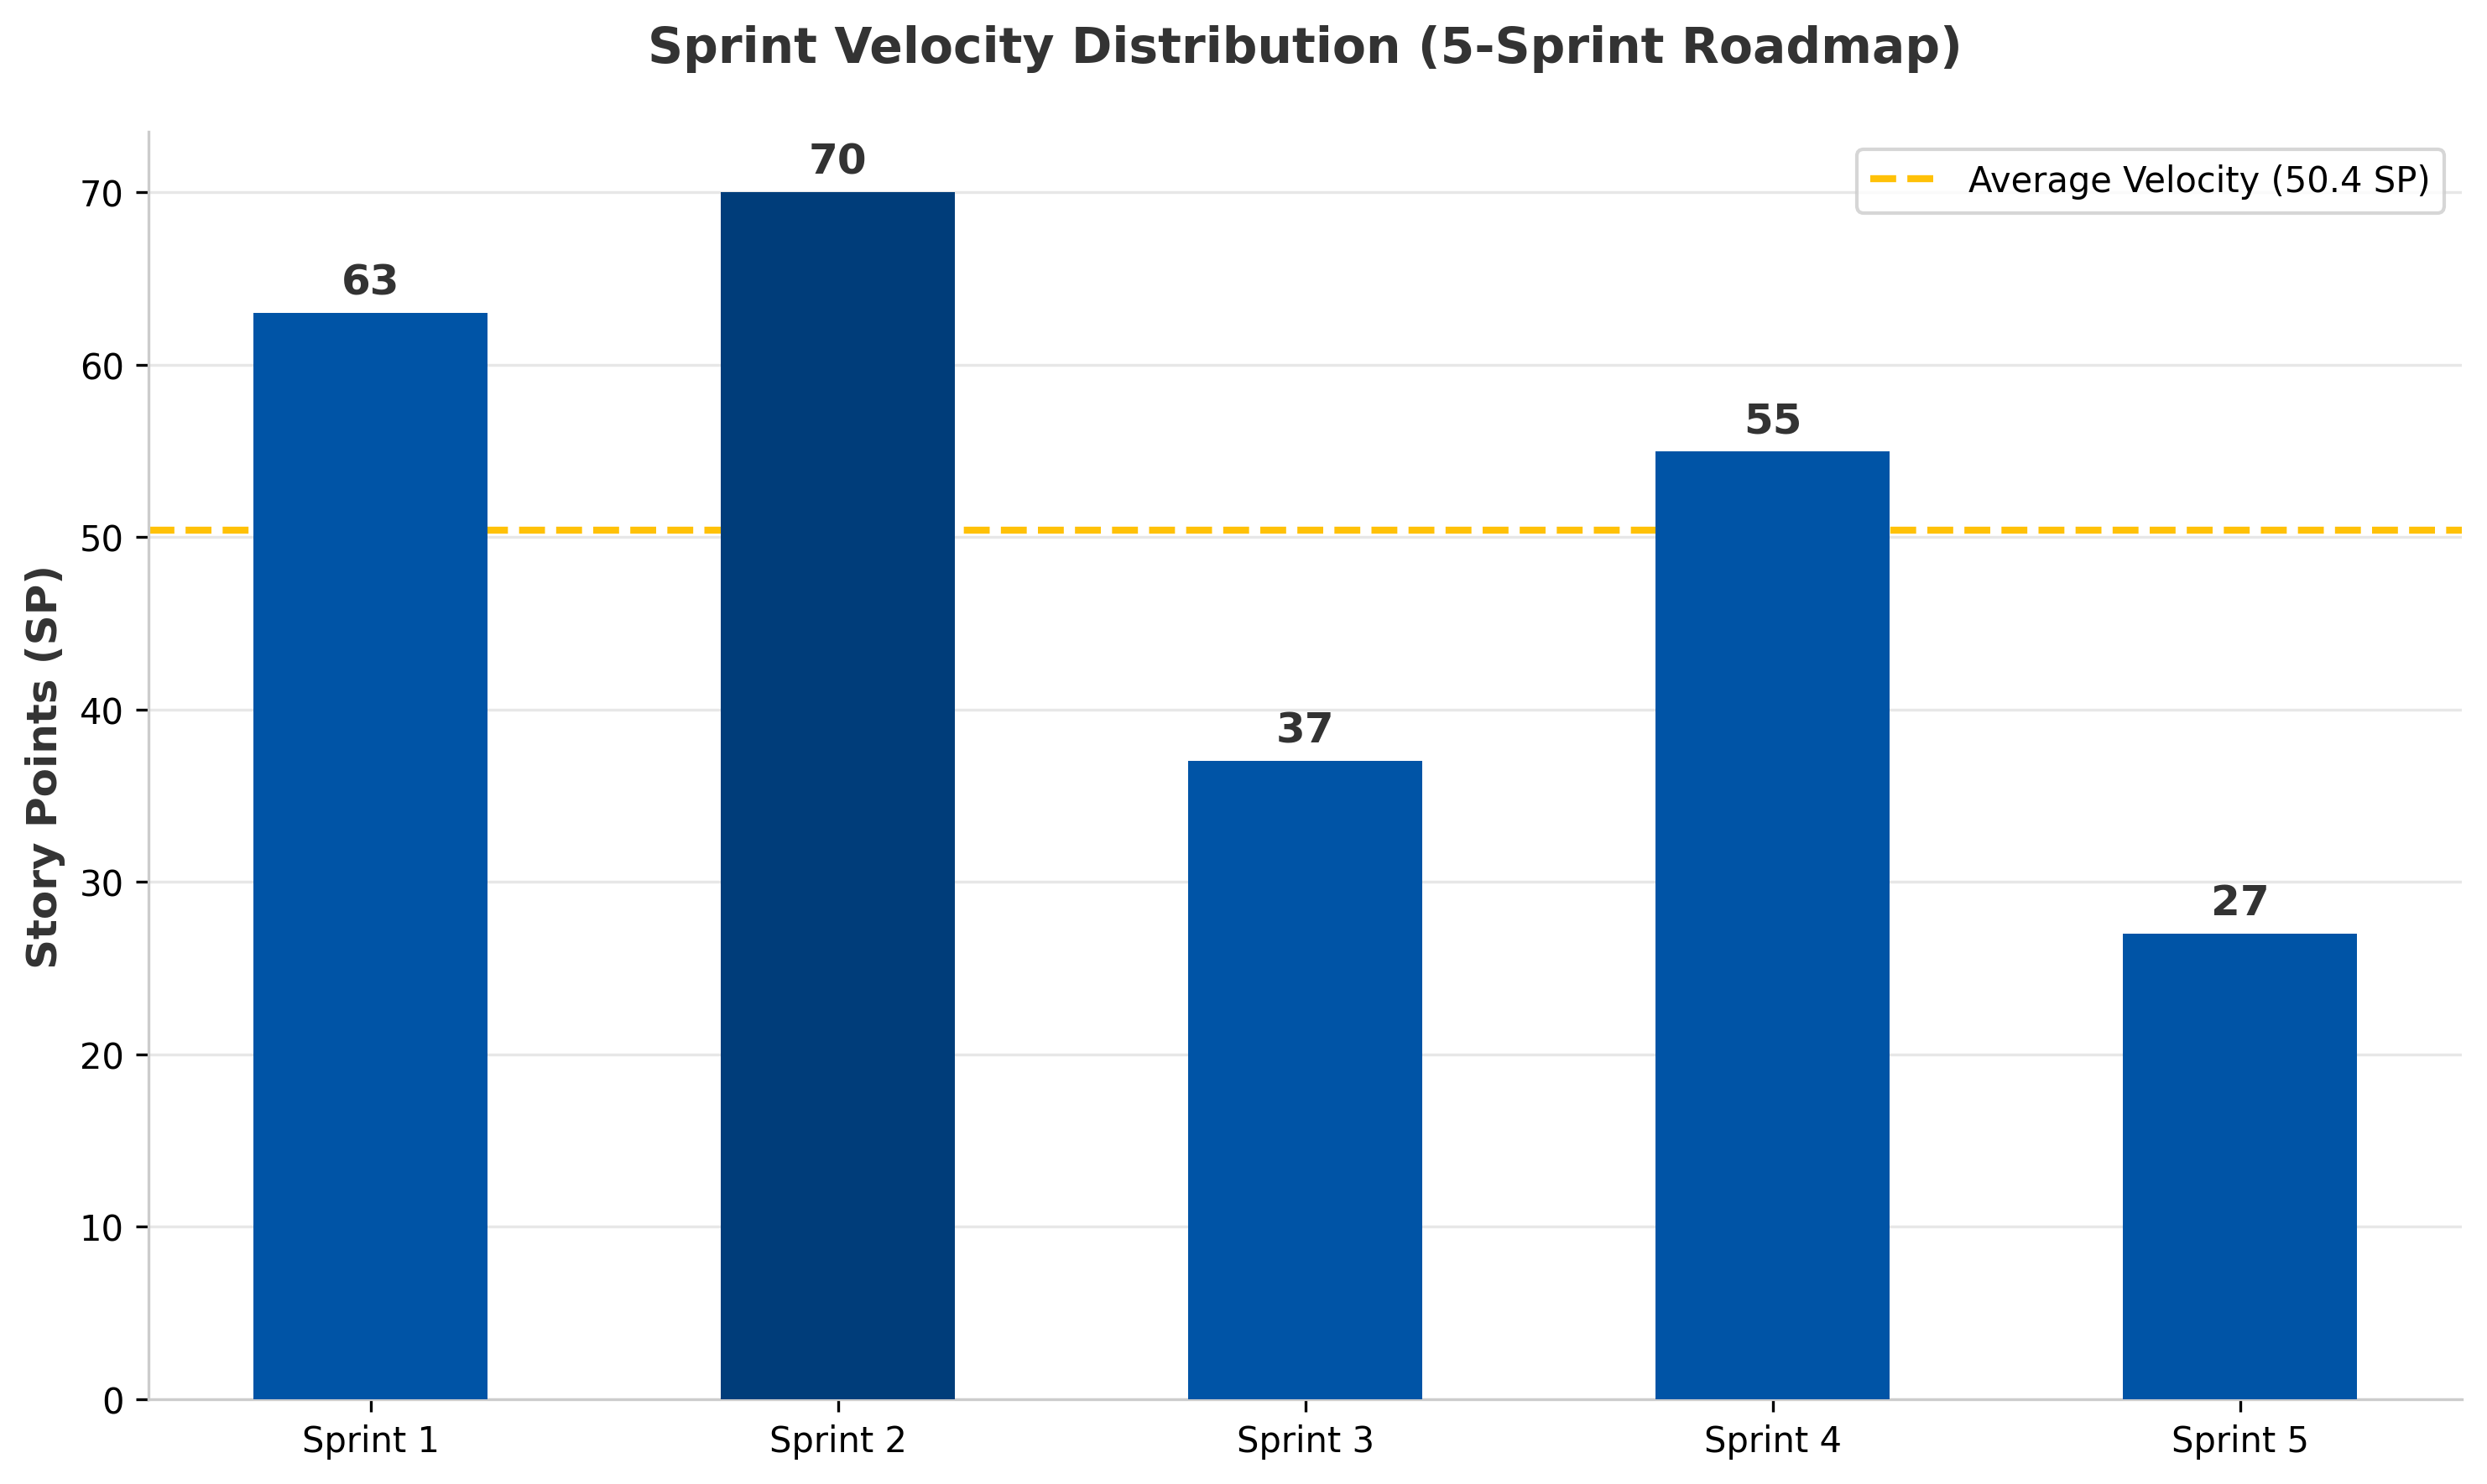
\includegraphics[width=0.75\textwidth]{images/sprint_velocity.png}
    \caption{Velocity distribution across the project lifecycle}
    \label{fig:sprint_velocity}
\end{figure}


\section*{Conclusion}
\addcontentsline{toc}{section}{Conclusion}

This chapter has transformed our project vision into a structured technical blueprint. By identifying our core actors and defining twenty-two rigorous requirements, we established a foundation centered on security and deterministic logic. Our Use Case and Sequence diagrams served as the final validation, mapping out the precise interactions that define the platform's behavior.

Finally, by organizing our 53-story backlog into five risk-assessed sprints, we created a clear and consolidated path for development. With the "what" and "why" firmly established, we are now ready to move into the implementation phase. The following chapter details the technical journey across these sprints, presenting the microservices architecture, the open-source technology stack, and the core development of each platform component.
